
\documentclass[10pt,a4paper]{article}
\usepackage[utf8]{inputenc}
\usepackage[french]{babel}
\usepackage[left=2cm,right=2cm,top=2cm,bottom=2cm]{geometry}
\usepackage{hyperref}
\usepackage{graphicx}

%opening
\title{TP}
\author{Nicolas Vadkerti}
\usepackage{listings} % Required for inserting code snippets
\usepackage[usenames,dvipsnames]{color} % Required for specifying custom colors and referring to colors by name

\definecolor{DarkGreen}{rgb}{0.0,0.4,0.0} % Comment color
\definecolor{highlight}{RGB}{255,251,204} % Code highlight color

\lstdefinestyle{Style1}{ % Define a style for your code snippet, multiple definitions can be made if, for example, you wish to insert multiple code snippets using different programming languages into one document
language=Perl, % Detects keywords, comments, strings, functions, etc for the language specified
backgroundcolor=\color{highlight}, % Set the background color for the snippet - useful for highlighting
basicstyle=\footnotesize\ttfamily, % The default font size and style of the code
breakatwhitespace=false, % If true, only allows line breaks at white space
breaklines=true, % Automatic line breaking (prevents code from protruding outside the box)
captionpos=b, % Sets the caption position: b for bottom; t for top
commentstyle=\usefont{T1}{pcr}{m}{sl}\color{DarkGreen}, % Style of comments within the code - dark green courier font
deletekeywords={}, % If you want to delete any keywords from the current language separate them by commas
%escapeinside={\%}, % This allows you to escape to LaTeX using the character in the bracket
firstnumber=1, % Line numbers begin at line 1
frame=single, % Frame around the code box, value can be: none, leftline, topline, bottomline, lines, single, shadowbox
frameround=tttt, % Rounds the corners of the frame for the top left, top right, bottom left and bottom right positions
keywordstyle=\color{Blue}\bf, % Functions are bold and blue
morekeywords={}, % Add any functions no included by default here separated by commas
numbers=left, % Location of line numbers, can take the values of: none, left, right
numbersep=10pt, % Distance of line numbers from the code box
numberstyle=\tiny\color{Gray}, % Style used for line numbers
rulecolor=\color{black}, % Frame border color
showstringspaces=false, % Don't put marks in string spaces
showtabs=false, % Display tabs in the code as lines
stepnumber=5, % The step distance between line numbers, i.e. how often will lines be numbered
stringstyle=\color{Purple}, % Strings are purple
tabsize=2
}

\newcommand{\insertcode}[2]{\begin{itemize}\item[]\lstinputlisting[caption=#2,label=#1,style=Style1]{#1}\end{itemize}} 


% \insertcode{"Scripts/example.pl"}{Nena would be proud.} 

\begin{document}

\maketitle


\url{https://github.com/SlaynPool/CR_Latex/}

\section{Écrire le script qui permet d’ouvrir le fichier de logauth.loget de comptabiliser le nombre de fois où’authentication failure’apparaît.}
\insertcode{code/1.py}{comptabiliser occurence}

 \section{Faire la même chose avec’Failed password for invalid user’}
 \insertcode{code/2.py}{Même chose}
 \section{Utilisation d'un dictionnaire et matplotlib}
 \insertcode{code/3.py}{Utilisation d'un dictionnaire}
 De là, si on veut chercher une nouvezlle chaine de character, il suffit de rajouter une entrée dans notre dictionnaire.
 On peut de là créer un graphique comme ceci :
 \insertcode{code/4.py}{Utilisation de matplotlib}
 \begin{figure}[h!]
\centering
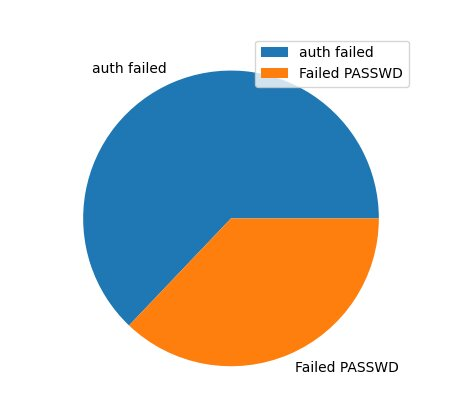
\includegraphics[scale=0.50]{image/1.jpg}
\caption{Graphique génerée }
\label{fig:net }
\end{figure}
\section{Adapter votre code pour produire un camembert relatif à vos calculs}
Ha ben ducoup, déja fait.

\section{En analysant vos fichiers de logs, ou celui de la machine web-mmiprésent sur Moodle, ajouter quelques informations supplémentaires à monitorer dans vos calculs}
Honnetement j'ai pas trop d'idée mais :
\insertcode{code/5.py}{Analyse des Failed as ROOT}

\section{Modifier votre programme Python pour pouvoir générer un tel rapport en LATEX.  Vous pourrez écrire un script Bash pour exécuter votre script Python puis compiler le fichier.tex généré à l’aide de la commande pdflatex}

 \insertcode{code/6.py}{Génération de PDF en python}

Voici un screen du rapport ainsi généré (le pdf est trouvable sur le git relatife au tp)

 \begin{figure}[h!]
\centering
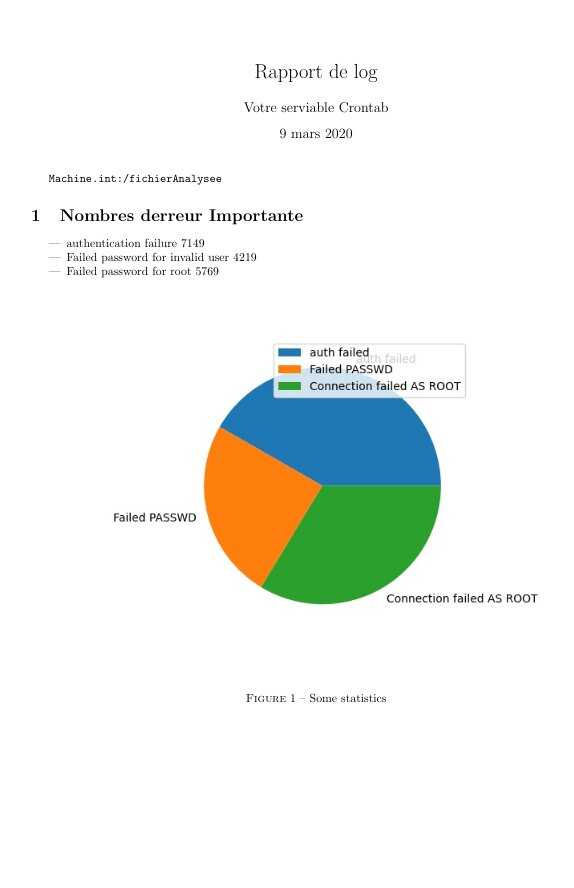
\includegraphics[scale=0.250]{image/2.jpg}
\caption{Rapport génerée }
\label{fig:net }
\end{figure}

\end{document}

